\newpage
\setlength{\parskip}{0cm}
\begin{Large}
\section{Анализ предметной области}
\subsection{Анализ аналогичных проектов}
В основе нейросетевых технологий лежит принцип искусственных нейронных сетей. Искусственная нейронная сеть - математическая модель, а также её программное или аппаратное воплощение, построенная по принципу организации и функционирования биологических нейронных сетей — сетей нервных клеток живого организма. Нейронные сети не программируются в привычном смысле этого слова, они обучаются. Возможность обучения — одно из главных преимуществ нейронных сетей перед традиционными алгоритмами. Технически обучение заключается в нахождении коэффициентов связей между нейронами[8]. Однако существует множество способов обучения нейронных сетей. 

Так, в одной статье рассматривается модель нейронной сети, имитирующей логику противника в игре «крестики-нолики»[1]. Структура разработанной сети состоит из одного входного нейрона, промежуточного слоя, состоящего из девяти нейронов, каждый из которых отвечает за клетку на поле, и выходного нейрона. Каждый промежуточный нейрон имеет свое весовое значение в пределах от - 1 до 1, от которого зависит выбор клетки для хода. Сеть оценивает каждую свободную клетку и выбирает наиболее перспективную. Обучающая выборка состоит из наборов заранее записанных ходов против сети. Нейронная сеть играет против каждого набора до тех пор, пока не выиграет. Процесс обучения состоит в том, что перед началом матча нейронная сеть генерирует значения весов. Исходя из этих значений и свободных клеток, сеть делает свои ходы, если она проигрывает игру значения весов, которые соответствуют произведенным ходам, уменьшаются. Если сеть выигрывает игру, значения весов увеличиваются, и игра записывается в память. Если сеть играет в ничью, то значения весов не изменяются, игра записывается в память, но дополнительно играет еще три раза с новыми значениями весов, для проверки возможности других комбинаций ходов. Процесс выбора связан с обращением сети к ее памяти значений весов. Находится игра из памяти, где противником были сделаны ходы, сделанные в текущей игре, но сеть при этом выиграла. Выбирается наиболее приближенное к единице значение весов, которое затем конвертируется в клетку. Автор отмечает что, если оппонент специально не поддаётся сети, то исходом матчей будет являться ничья, как и в случае, если нейронная сеть будет играть против такой же нейронной сети.

В другой статье рассматривается реализация поведения агента в мультиагентной компьютерной игре[4]. Игра “Collector Stars” представляет собой двумерную игру в жанре платформер для одного или нескольких игроков. Игра представлена двумерной сеткой ячеек разного типа: проходимая, непроходимый блок, звезда, черная дыра и дверь. Персонажу Собирателю нужно найти выход из уровня, попутно собирая звезды и избегая черных дыр. Агент-собиратель может перемещаться влево или вправо и прыгать на высоту, чуть выше, чем высота одной ячейки карты.  Имеет меньшие размеры по ширине и высоте, чем размер ячейки.

На вход искусственной нейронной сети подается набор атрибутов текущего состояния. Значение первого входа зависит от того, находится ли персонаж на блоке, и может иметь значение ноль или единица. Второй и третий входы представляют значения компонент нормированного вектора скорости Собирателя. Третий и четвертый входы представляют значения компонент нормированного вектора направления ближайшего противника. Пятый и шестой - координаты центра Собирателя относительно ячейки, в которую входит точка центра. Координаты нормируются с учетом размера ячейки. Далее следуют входы, представляющие ячейки вокруг собирателя, их количество определялось при тестировании. Выходом сети будут три значения, исходя из которых будут определены действия Собирателя: движение влево, вправо и прыжок, соответственно. Действие будет активизировано, если полученное значение больше 0.5.
\subsection{Обзор методов обучения нейронной сети}
Обучение на основе учебной выборки для игры в монополию невозможно, ввиду огромного количества вариантов развития. Однако существуют другие варианты обучения нейронной сети. Так в статье[4] был выбран эволюционный подход с помощью генетического алгоритма. Для обучения таким способом гены хромосом определяются как вес всех связей нейронной сети. На этапе инициализации хромосомы заполняются случайными вещественными числами из интервала [-1,1]. Агент использует значения хромосом для задания весов сети. Для определения приспособленности каждой хромосомы агенту дается некоторое время на прохождение уровня. Агент будет проходить уровень столько раз, сколько хромосом в популяции. После окончания времени, гибели или пересечения двери, приспособленность определяется как количество набранных очков. Причем если Собиратель погиб, очки все равно будут вычисляться по этой формуле, но будет использоваться количество итераций, даваемое на прохождение. После вычисления приспособленности, выполняются остальные шаги алгоритма.

Селекция или выбор родителей: метод рулетки. Каждой хромосоме сопоставляется значение, величина которого устанавливается пропорционально значению приспособленности данной хромосомы. Чем больше значение приспособленности, тем больше вероятность ее выбора.

Скрещивание и мутация: скрещивание выполняется одноточечным обменом, мутация для каждого гена происходит с вероятностью 0.01. Значение гена меняется путем прибавления случайного числа из отрезка [-0.3; 0.3] и ограничивается отрезком [-1;1].

Выбор следующего поколения: из старого поколения берется 0.6 лучших по приспособленности особей. Они объединяются с полученными потомками, но с сохранением размера популяции (т. е. часть потомков не попадет в новое поколение).

Автор приводит сравнение с другими алгоритмами, из которых видно, что нейронная сеть набирает наибольшее количество очков, однако обучается и проходит уровень чуть дольше чем алгоритм R-Learning.

Помимо лучшей скорости обучения, алгоритм Reinforcement Learning превосходно подходит для случаев, где рассматриваемая система является марковским случайным процессом, то есть процессом «будущее» которого не зависит от «прошлого» при известном «настоящем». Основная идея reinforcement learning описана в статье[6]. Авторы рассматривают применение алгоритма обучения с подкреплением на примере игр приставки Atari, каждая из игр которой подходит под определение марковского случайного процесса. То есть находясь в состоянии s и выполняя действие a, которое входит в набор возможных действий, игра может выдать reward или сообщить об проигрыше. Вводится понятие cumulative return over time – общее количество reward, которое алгоритм может получить от текущего момента до конца игры. Помимо этого, reward с каждым шагом системы уменьшается на константу $\gamma$. Оптимальное поведение при данных обстоятельствах можно описать функцией Q*(s,a), цель которой достигнуть максимального cumulative return over time. Данная функция называется Bellman Equation и выглядит данным образом:
\begin{figure}[h]
    \center{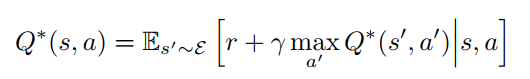
\includegraphics[width=1\linewidth]{bellman}}
    \caption{Bellman Equation - функция поведения игрока}
\end{figure}

Помимо этого, с определённой вероятностью, которая уменьшается после каждой игры, вместо наиболее выгодного действия выбирается случайное из возможных. После каждой игры выбираются случайные наборы действий для корректировки весов нейронной сети, то есть основная задача нейронной сети предсказать какое действие приведёт к максимальному значению Q функции в следующий момент времени. Данный метод называется Q-Learning. После реализации алгоритма авторы статьи сравнили полученные результаты с результатами других способов обучения искусственного интеллекта. Q-Learning в большинстве игр оказался лучшим.
\subsection{Обзор существующих технологий для реализации проекта}
В связи с развитием машинного обучения в последние годы появилось множество вспомогательных библиотек, которые инкапсулируют реализацию моделей нейронной сети, позволяя очень быстро протестировать идею без постоянного написания основного каркаса нейронной сети.

Одной из самых популярных библиотек машинного обучения является TensorFlow[9], разрабатываемая компанией Google. TensorFlow – это программная библиотека с открытым исходным кодом для численных вычислений с использованием графов потоков данных (data flow graphs). Узлы в таком графе представляют математические операции, в то время, как грани представляют передачу данных (многомерных массивов) между узлами. Гибкая архитектура, на основе которой построен TensorFlow, позволяет разворачивать вычисления на одном или нескольких CPU или GPU (т.е. на центральном или графическом процессоре) на обычном персональном компьютере, сервере или даже мобильном устройстве используя единый программный интерфейс (API).  В одной из статей рассматриваются основные возможности данного программного решения[2]. Автор реализует логистическую регрессию и сравнивает время выполнения с результатом библиотеки scikit-learn. TensorFlow оказывается гораздо быстрее – 17c против 3 мин., и точнее в предсказании на тестовой выборке – 92% против 91.8%. На данном примере отмечается, что принципиальным отличием TensorFlow (далее – TF) от scikit-learn в том, что определение порядка вычислений и собственно само вычисление разнесено на отдельные шаги, т.е., определяя последовательность действий в TF, на самом деле формируется граф операций, а само вычисление графа будет происходить позже, на уже конкретных физических устройствах (CPU, GPU или отдельных компьютерах), что приводит к ускорению вычислений. 

Далее автор реализует feed-forward нейронную сеть, отмечая, что основная сложность нейронных сетей заключена в обратном распространении ошибки, однако, работая с TF об этом не приходится задумываться, потому что в нем реализован обобщенный алгоритм обратного распространения ошибки, т.е. такой алгоритм, который применим к любым доступным операциям (будь то умножение матриц или операция свертки для свёрточных нейронных сетей). Для обучения используется 55000 изображений, для валидации 5000, в качестве тестовой выборки 10000 изображений. В результате выполнения отмечается, что TensorFlow выполняется в 6 раз быстрее библиотеки Theano. Помимо этого, TensorFlow предоставляет встроенные средства визуализации, которые повышают наглядность обучаемых моделей.

Несмотря на то, что TensorFlow подходит как для широкого набора техник машинного обучения, так и для глубинного обучения, библиотека может быть довольно сложна в понимании особенно для тех разработчиков, которые только начинают знакомство с данными областями исследования. Альтернативой является «надстройка» Keras [10], которая предоставляет удобный и простой в использовании программный интерфейс для обучения глубоких нейронных сетей. Keras не является самостоятельной системой, а работает поверх Theano, TensorFlow или CNTK. В 2016 году Keras включили в состав TensorFlow[10]. Помимо этого, все классы являются максимально расширяемыми и модульными, благодаря этому библиотека представляет широкий функционал возможностей по решению сложных практических задач.
\subsection*{Выводы}
\addcontentsline{toc}{subsection}{Выводы}
В результате обзора литературы были изучены различные реализации нейронных сетей для построения логики игрового противника. Игра в монополию является марковским случайным процессом [7], следовательно, для обучения искусственного интеллекта был выбран алгоритм Q-Learning.

Были рассмотрены основные средства реализации нейронных сетей в языке Python, в результате чего была выбрана реализация с применением библиотеки Keras.
\end{Large}